\problemname{Milling Machines}

\illustration{.4}{mm.jpg}{Photo by aurelie ghalim on Flickr}%
A fab lab is an open, small-scale workshop where you
can create or fabricate almost anything you want mostly by using computer
controlled tools like a laser cutter or a 3D printer.
The FAU fab lab recently got a CNC milling machine. Using the milling machine
you can cut or remove material with different tools from the surface of a
workpiece. It is controlled via a computer program.

I sometimes wondered what happens if multiple different shaped
workpieces are sent through the same milling program. For simplification assume that we
have only two dimensional workpieces without holes. A milling program consists of
multiple steps; each step describes where the milling machine has to remove
material (using different tools) from the top of the surface.


\section*{Input}
The first line consists of two integers $W$ and $S$, where $W$ gives the number
of workpieces and $S$ the number of steps in the milling program ($1 \le W, S \le
10^{4}$).
The next line consists of two integers $X$ and $Y$, where $X$ gives the
width and $Y$ gives the maximal possible height of workpieces ($1 \le X, Y
\le 100$).\\
Then follow $W$ lines, each describing one workpiece. Each workpiece
description consists of $X$ non-negative integers specifying the surface height
in that column.\\
Then follow $S$ lines, each describing one milling step of the milling progam.
Each milling step description consists of $X$ non-negative integers $s_i$ ($0 \le s_i \le Y$) specifying
the amount of surface to cut off in each column (relative to the height of
the milling area, i.e.\ $Y$, not relative to the top of the workpiece). See Fig.~\ref{figmill} for details.

\section*{Output}
For each workpiece, output one line containing  $X$ integers specifying the
remaining surface heights (in the same order as in the input).
\begin{figure}[h]
	\vspace*{-1em}
	\centering
	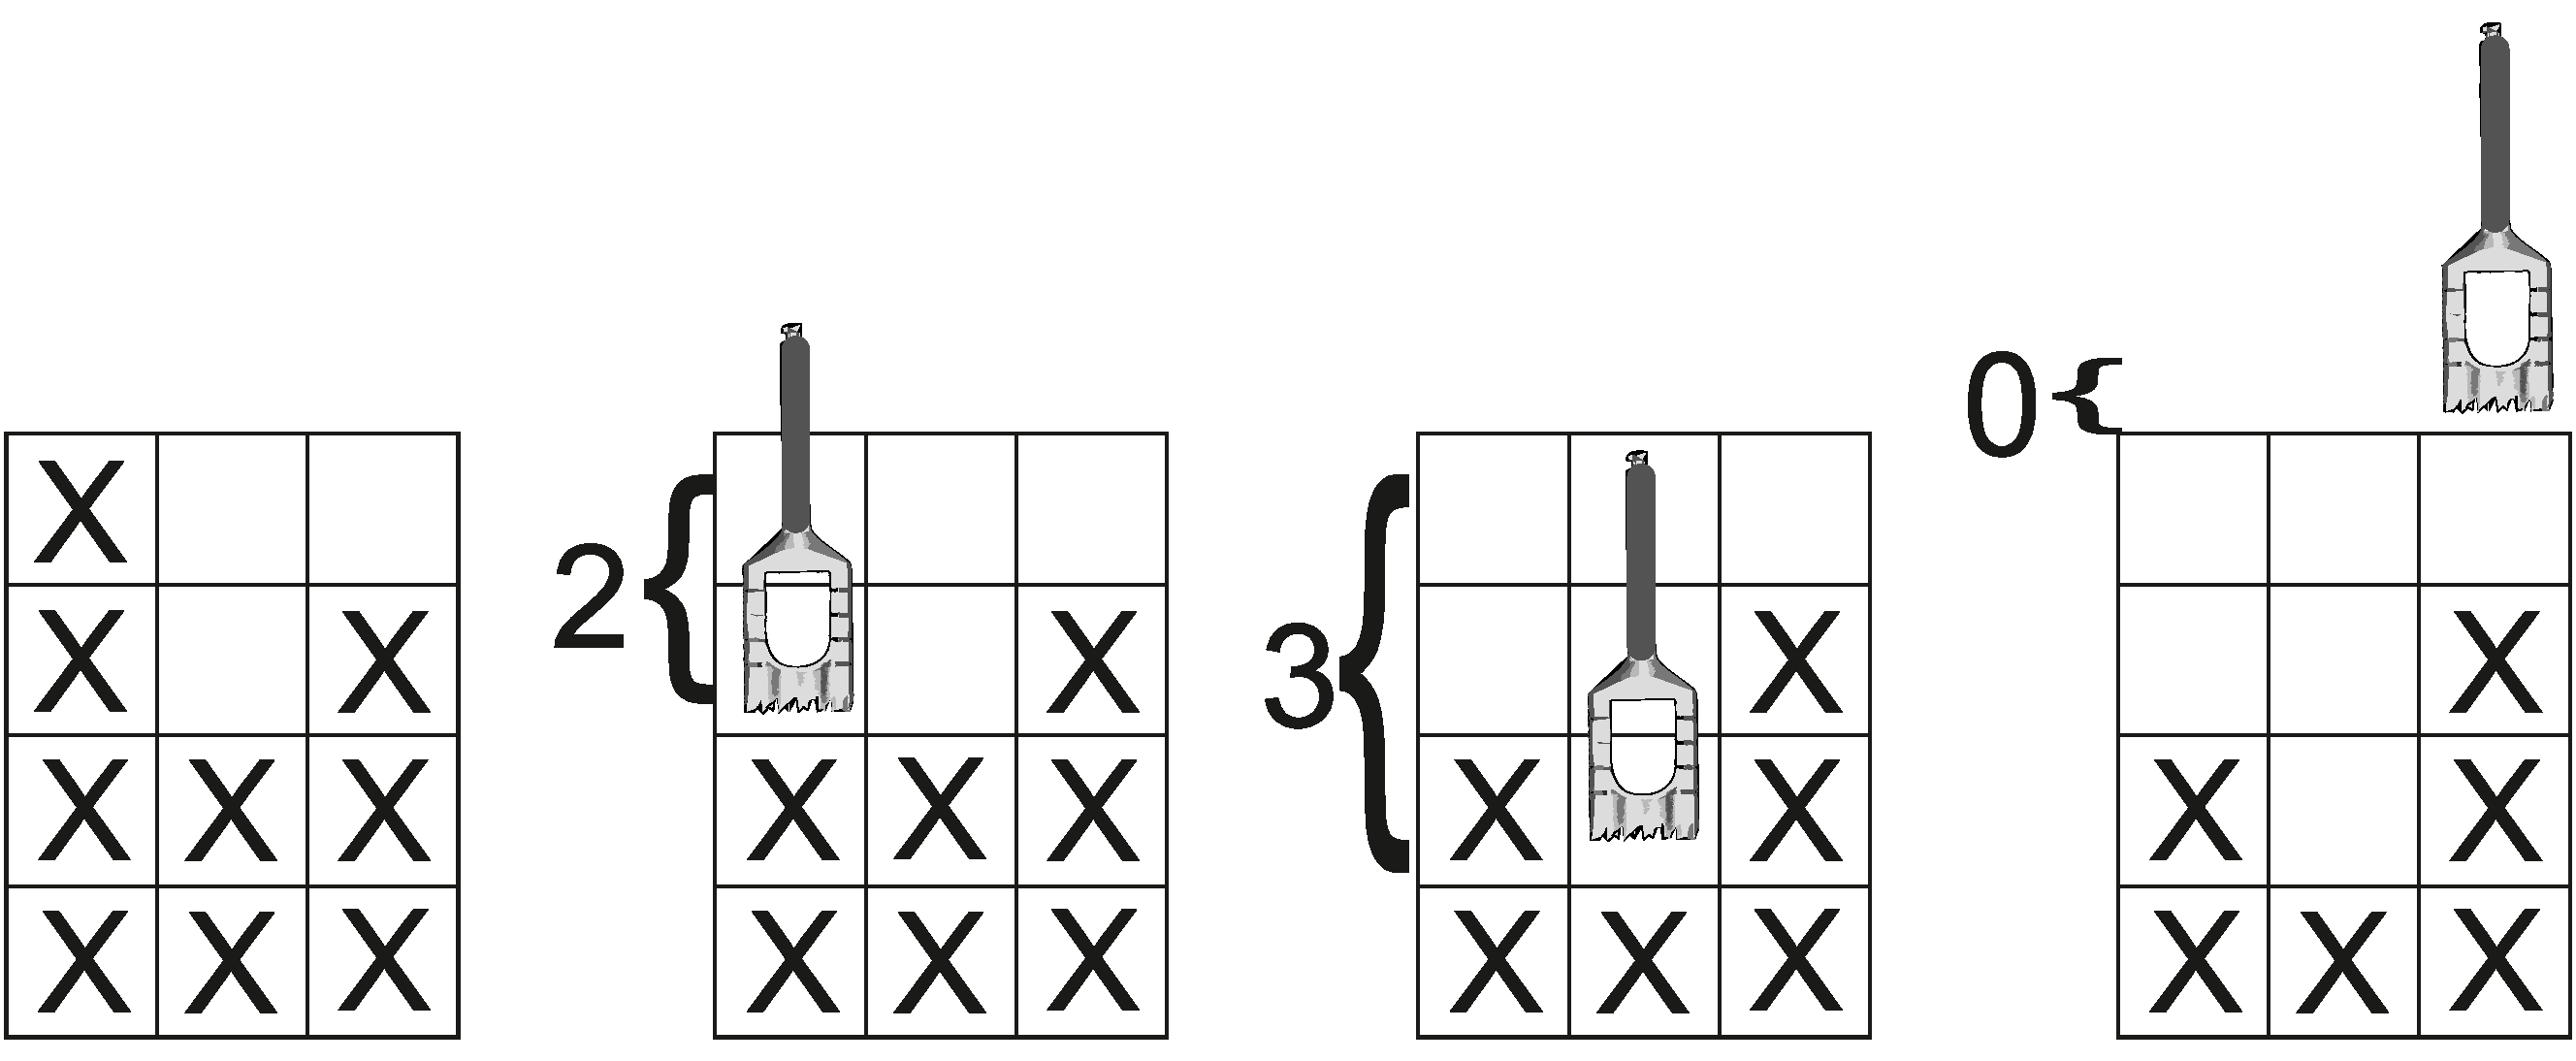
\includegraphics[width=.45\textwidth]{milling.pdf}
	\caption{Second workpiece in first sample: initial workpiece followed by milling in each column -- the value in the milling program determines the vertical position of the cutter head.\label{figmill}}
\end{figure}
